%
% File Name     : Protokoll.tex
% Purpose       :
% Creation Date : 02-12-2013
% Last Modified : Tue 03 Dec 2013 02:02:49 PM CET
% Created By    :
%

\documentclass[a4paper,12pt]{article}
\usepackage{amsfonts}
\usepackage{listings}
\usepackage{tabularx}
\usepackage[utf8]{inputenc}
\usepackage[ngerman]{babel}
\usepackage{fancyhdr}
\usepackage{amsmath}
\usepackage{graphicx}
\usepackage[hidelinks]{hyperref}
\usepackage{biblatex}

\pagestyle{fancy}

\fancyhead[R]{\today}
\fancyhead[L]{Datenbanken}


\begin{document}
\title{Labor Datenbanken Gruppe 10}
\author{ Oliver Gebhard \and Dominik Glienke }
\maketitle

\newpage
\tableofcontents
\newpage
\setcounter{tocdepth}{2}


\section{Einleitung}

\begin{figure}[h]
    \centering
    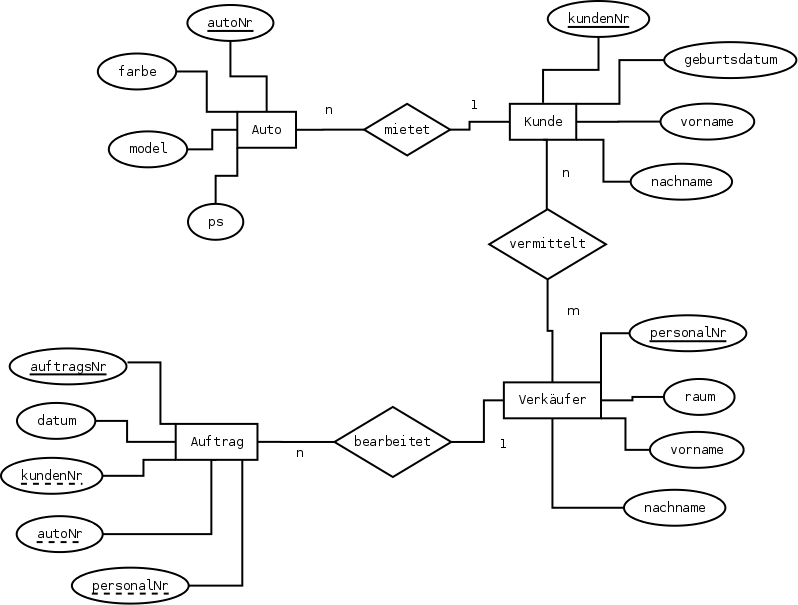
\includegraphics[scale=0.34]{ER_Schema_Autovermietung.png}
    \caption{ER-Schema}
    \label{Autovermietung}
\end{figure}

\subsection{Beschreibung}

ER-Schema Autovermietung \\

Folgendes ER-Schema stellt Geschäftsprozesse der Autovermietung im Groben dar. 
Das Entity 	Auto besitzt die Attribute autoNr (Primärchlüssel), farbe, model, ps.
		Kunde besitzt die Attribute kundenNr (Primärschlüssel), geburtsdatum, vorname, nachname.
Verkäufer besitzt die Attribute personalNr (Primärschlüssel), raum, vorname, nachname.
Auftrag besitzt die Attribute auftragsNr (Primärschlüssel), datum, sowie die Fremdschlüssel kundenNr, autoNr, personalNr.

Zwischen Kunde und Auto besteht eine 1:n-Beziehung. Das heißt, dass ein Kunde (theoretisch) beliebig viele Autos mieten kann. Gleichzeitig kann ein Auto nur von einem Kunden gleichzeitig gemietet werden.
Zwischen Kunde und Verkäufer besteht eine n:m-Beziehung. Ein Kunde kann mehrere Verkäufer haben, die diesem Fahrzeuge vermitteln, gleichzeitig kann ein Verkäufer mehrere Kunden haben.
Zwischen Verkäufer und Auftrag besteht eine 1:n-Beziehung, denn ein Verkäufer bearbeitet beliebig viele Aufträge aber ein Auftrag kann nur von einem Verkäufer bearbeitet werden.

\newpage
\begin{appendix}
\section{Anhang}

\subsection{SQL}

\lstinputlisting[language=SQL]{statements.sql}

\end{appendix}

\end{document}
